\documentclass[10pt,a4paper]{article}
\usepackage[utf8]{inputenc}
\usepackage{amsmath}
\usepackage{amsfonts}
\usepackage{amssymb}
\usepackage{graphicx}
\usepackage{url}
\usepackage{listings}

\usepackage{color}

\definecolor{mygreen}{rgb}{0,0.6,0}
\definecolor{mygray}{rgb}{0.5,0.5,0.5}
\definecolor{mymauve}{rgb}{0.58,0,0.82}

\lstset{ %
  backgroundcolor=\color{white},   % choose the background color; you must add \usepackage{color} or \usepackage{xcolor}
  basicstyle=\footnotesize,        % the size of the fonts that are used for the code
  breakatwhitespace=false,         % sets if automatic breaks should only happen at whitespace
  breaklines=true,                 % sets automatic line breaking
  captionpos=b,                    % sets the caption-position to bottom
  commentstyle=\color{mygreen},    % comment style
  deletekeywords={...},            % if you want to delete keywords from the given language
  escapeinside={\%*}{*)},          % if you want to add LaTeX within your code
  extendedchars=true,              % lets you use non-ASCII characters; for 8-bits encodings only, does not work with UTF-8
  frame=single,                    % adds a frame around the code
  keywordstyle=\color{blue},       % keyword style
  language=Octave,                 % the language of the code
  morekeywords={*,...},            % if you want to add more keywords to the set
  numbers=left,                    % where to put the line-numbers; possible values are (none, left, right)
  numbersep=5pt,                   % how far the line-numbers are from the code
  numberstyle=\tiny\color{mygray}, % the style that is used for the line-numbers
  rulecolor=\color{mygray},         % if not set, the frame-color may be changed on line-breaks within not-black text (e.g. comments (green here))
  showspaces=false,                % show spaces everywhere adding particular underscores; it overrides 'showstringspaces'
  showstringspaces=false,          % underline spaces within strings only
  showtabs=false,                  % show tabs within strings adding particular underscores
  stepnumber=2,                    % the step between two line-numbers. If it's 1, each line will be numbered
  stringstyle=\color{mymauve},     % string literal style
  tabsize=2                       % sets default tabsize to 2 spaces
%  title=\lstname                   % show the filename of files included with \lstinputlisting; also try caption instead of title
}

%TODO: The V model.

\begin{document}

\author{
  Ibrahim Nemli (s093477@student.dtu.dk)\\
  Søren Tidemand Møller Harving (s093472@student.dtu.dk) \\
  Kim Rostgaard Christensen (kroch@imm.dtu.dk)
}
\title{02241 - Robust software systems \\
	First draft
}

\maketitle

\begin{abstract}
A robust software system can be described as a system which aims to be unbreakable in several situations. Unbreakable does not mean that the system has not got any errors, but the errors that may occur are handled in a way, so that the system returns an understandable description of the error to the user, fails in a safe manner or possibly degrade to a lower level of functionality. However, robustness in general and indeed with regards to software is difficult to define and quantify.
\end{abstract}

\tableofcontents

\begin{figure}[h]
\centering
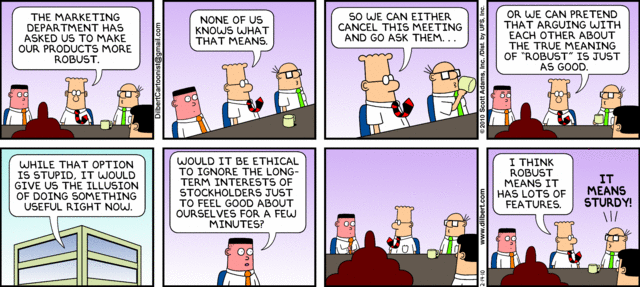
\includegraphics[scale=0.4]{fig/dilbert_robust.png}
 \caption{The Dilbert take on robustness (License: grey area)}
 \label{fig:dilber_robustness}
\end{figure}

\newpage
\section{Defining robustness}
As figure \ref{fig:dilber_robustness} states, robustness can be a fuzzy term which is sometimes over-sold by egar marketeers.
However, there exist several engineering disciplines that focus on robustness individually. The fields covered here are;
\begin{itemize}
\item Safety
\item Security
\item Resilience
\item Usability
\end{itemize}
While they are not mutually exclusive fields of engineering, they each have their own set of parameters to optimize.

\subsection{Safety engineering}

Seeks to optimize on factors that provide maximum safety, typically by focusing on the absence of errors or unsafe procedures. Safety can also be be provided by the use of barriers which in general can be realized by, for instance, physical obstacles such as walls or fences, or merely regulations or safety standards (including legislations).
For the software world, barriers can be implemented by either coding standards, or language restrictions (e.g. sub-setting). Extensive testing is also applicable as it gives some confidence that a system is safe within the bounds of the test environment.

\subsection{Security engineering}

Is mainly concerned with the issue of keeping a system out of harms way by preventing malicious users (or programs) in misusing it.
Robustness in this meaning will be the absence of security breaches, strong authentication mechanisms and appropriate internal ACL’s\footnote{Access Control List}.
Security can be defined on numerous levels, from the hardware layer to the physical world - by hindering access to systems altogether.

\subsection{Resilience engineering}
Whereas safety engineering takes the high road of idealism, building systems that never breaks. Resilience engineering takes the low road of acceptance, embracing the fact that there are no perfect systems, or unsinkable ships to take an example.
The main parameter targeted for optimization here is fault tolerance, and the goal is to provide fault-tolerance and, where applicable, a fail-safe system.
In software systems, this is typically realized by adding redundant components or extra information to data\cite{KoKr07}
. This could be checksums/parities or validation schemas, such as DTD’s\footnote{Document Type Definition} for XML.

\subsection{Usability engineering}

Although not a robustness-specific field, more and more evidence suggest that bad and counter-intuitive human interfaces leads to bad decisions, which then again lead to system failures.
Usability engineering deals with what can be described as as applied joint cognitive systems\cite{hollnagel2005joint} engineering, where the user interface of a system is not treated as a boundary layer, but more as a complete system \emph{containing} the human operator.
The goal is, in brief, to provide the right information, no more or less, at the right time to the user, and the appropriate methods of control.

\subsection{Summary}
Clearly, there are a lot of interests in improving the robustness of a software system, be the motivator either constant loss of data from word-processing application, or securing a nuclear power plant from melting down, everyone likes their software responsive, correct and robust.

\section{Programming principles}

To help the programmer to build a robust software system, he or she can use the principles explained below.

\subsection{Programming defensively}

Programming defensively is one of the essential techniques in robust programming.
This is a method for ensuring that the software is functioning in every kind of unforeseeable usage of the program. In other words, we have to assume that the user wants to break the software by inserting in any kind of absurd, incorrect or malformed inputs, which would cause an error in the program. In all those cases, the program should not be vulnerable for those kind of inputs. The program should be able to print verbose and reasonable error messages in which the user can react upon.
Even there is a detailed documentation of how the program should be used, we cannot expect that the user has read it. If so we cannot even ensure that, the user has fully understood the documentation.\\

It is difficult to write perfect code (maybe impossible) but you can take advantages of defensive programming in terms of improving the quality of the code. This will reduce the amount of bugs, since the source code has been written in such way that it behaves in a predictable manner despite all kinds of errors that could occur.
One could say that the aim in defensive programming is to reduce the amount of errors that could happen.

\subsection{Information hiding}

In this case, we have to hide data as much as possible and only give enough information which has been asked for.
This can be implemented by having well-defined interfaces through which the program can access the information needed.
In object-oriented programming languages, we have the term encapsulation. This is a technique for restricting the access to some of the object’s components. In this way we can make sure that none of the internal component for an object can be reached and manipulates from outside.
By hiding data as described above, we prevent users from manipulating data and in that way destroying other data intentionally which the users as not supposed to have access to.

\subsection{Assume the impossible}

In order to have robust software systems you have to take care of cases, which look like that never can happen, since they often will happen (e.g. in a different environment than the original environment where the code has been developed). Those cases are based on our expectation on how the program is going to be utilized and executed. If our expectations are not fulfilled regarding to the usage, then the program will crash. Therefore, the programmer may not omit to take care of those kinds of cases.
 
This is one of the most difficult concept to learn in that it requires a great knowledge of the scenarios where the program is going to be used.
Another perspective in this principle is that our code is not fixed. We have to know that the source code may be changed during maintenance or expanding its functionality. Those changes might affect other parts of the software, which may lead to impossible cases occurring. 

\subsection{Contract programming}
Contract programming is a more exotic method for verifying the correctness of software.
The basic idea is that by adding additional semantics to your code, software tools can be used to prove whether or not a given procedure lives up to it's contract.
Consider the following prototype:
\lstinputlisting[frame=single, language=Ada] {include/Overflow_Example.adb}
The annotation specifies which conditions must be true upon entering the method (pre) and exiting (post). If we were to program the method so that X was decremented, or untouched, the verification software would fail and leave us with no option but to fix the bad implementation.
Contract programming is typically only used in safety-critical systems that mandates formal requirements for software correctness. Contracts and verification reports can be used as argument and documentation that the software is indeed correct - according to specifications.

\section{Implementation}

\subsection{Choice of Ada}
The background for choosing Ada is based on the assumption, or more precisely; claim, that programs written in Ada in general has less defect than other languages.

\appendix

% The following two commands are all you need in the
% initial runs of your .tex file to
% produce the bibliography for the citations in your paper.
\bibliographystyle{plain}

% These are entries that should be a part of references, no matter if they were cited or not.
\nocite{Chapman:2006:CCM:1151816.1151820}
\nocite{bishop2004teaching}
\nocite{Wikipedia:Defensive_programming}
\nocite{Wikipedia:OO_encapsulation}
\bibliography{references}  % sigpr

\end{document}